\documentclass[a4paper, 11pt]{article}
\usepackage[utf8]{inputenc}
\usepackage[ngerman]{babel}
\usepackage[T1]{fontenc}
\usepackage{graphicx}
\usepackage{float}
\usepackage{amsmath}
\usepackage{amssymb}
\usepackage{amsthm}
%\usepackage[paper=a4paper,margin=35mm]{geometry}

\newcommand{\W}{\operatorname{W}}

\title{AD -- Übungsblatt 8}
\author{Simon Thelen}

\begin{document}

\maketitle

\section*{Aufgabe 1}

\subsection*{1}
\begin{proof}
    Sei $k$ ein Knoten mit zwei Nachfolgern. Dann liegt der Inorder-Nachfolger $n$ von $k$ innerhalb des Teilbaums mit dem rechten Nachfolger von $k$ als Wurzel.
    Der Inorder-Nachfolger $n$ ist der Knoten mit dem kleinsten Wert $\W(n)$, der größer ist als $\W(k)$.
    $n$ kann keinen linken Nachfolger $l$ haben, denn es müsste $\W(k) < \W(l) < \W(n)$.
    Da jedoch $n$ der Inorder-Nachfolger ist, kann es im Baum keinen Wert zwischen $\W(k)$ und $\W(n)$ geben.
    Somit hat $n$ maximal einen Nachfolger.
\end{proof}

\subsection*{2}
\begin{proof}
    Gegeben sei der AVL-Baum mit Inorder-Darstellung
    \begin{equation*}
        (((n, 1, n), 2, n), 3, ((n, 4, n), 5, (n, 6, (n, 7, n))))
        \text{.}
    \end{equation*}
    Wird in dieser Reihenfolge \texttt{Delete(7)} und \texttt{Delete(4)} aufgerufen, ergibt sich der Baum
    \begin{equation*}
        (((n, 1, n), 2, n), 3, (n, 5, (n, 6, n)))
        \text{.}
    \end{equation*}
    Geschehen die beiden \texttt{Delete}-Aufrufe jedoch umgekehrt, ist der resultierende Baum
    \begin{equation*}
        (((n, 1, n), 2, n), 3, ((n, 5, n), 6, n)
        \text{,}
    \end{equation*}
    da bei letzterer Variante beim Löschen von \texttt{4} eine Linksrotation stattfindet, die bei Variante~1 fehlt.

    Damit wurde ein Gegenbeispiel, bei der AVL-Baum keine Kommutativität besitzt, gefunden und die Aussage widerlegt.
\end{proof}

\section*{Aufgabe 2}

\subsection*{1}
\begin{figure}[H]
    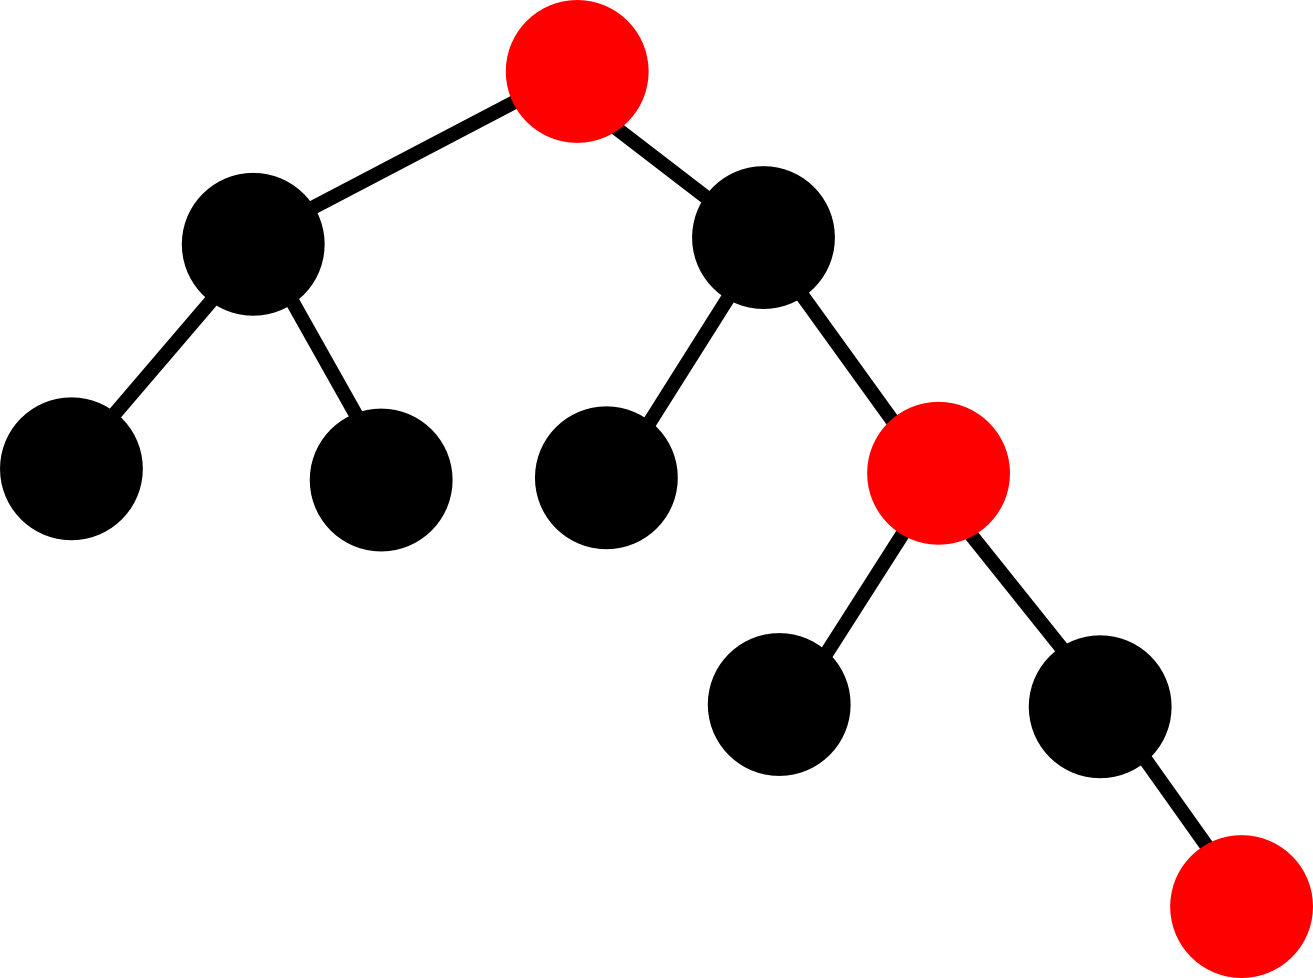
\includegraphics[width=8cm]{minimal_tree}
    \centering
\end{figure}

\subsection*{2}
\begin{proof}
    Bei einem Rot-Schwarz-Baum muss jeder Pfad eines Knoten zu seinen Blättern die gleiche Anzahl an schwarzen Knoten enthalten.
    Bei einem perfekt ausballancierten Rot-Schwarz-Baum wäre jeder Knoten schwarz.
    Damit also von einem Knoten ein Pfad zu einem Blatt länger wird als ein anderer Pfad, muss man rote Knoten einfügen.
    Da jedoch ein Knoten nur rot sein kann, wenn beide seiner Nachfolger schwarz sind, kann auf einem Pfad zu einem Blatt höchstens jeder zweite Knoten rot sein.
    Da ein Pfad mit roten Knoten aber natürlich immer noch genauso viele schwarze Knoten enthalten muss wie ein Pfad ohne rote Knoten, kann der Pfad mit roten Knoten höchstens doppelt so lang sein wie der ohne.
\end{proof}

\section*{Aufgabe 3 und 4}
\begin{figure}
    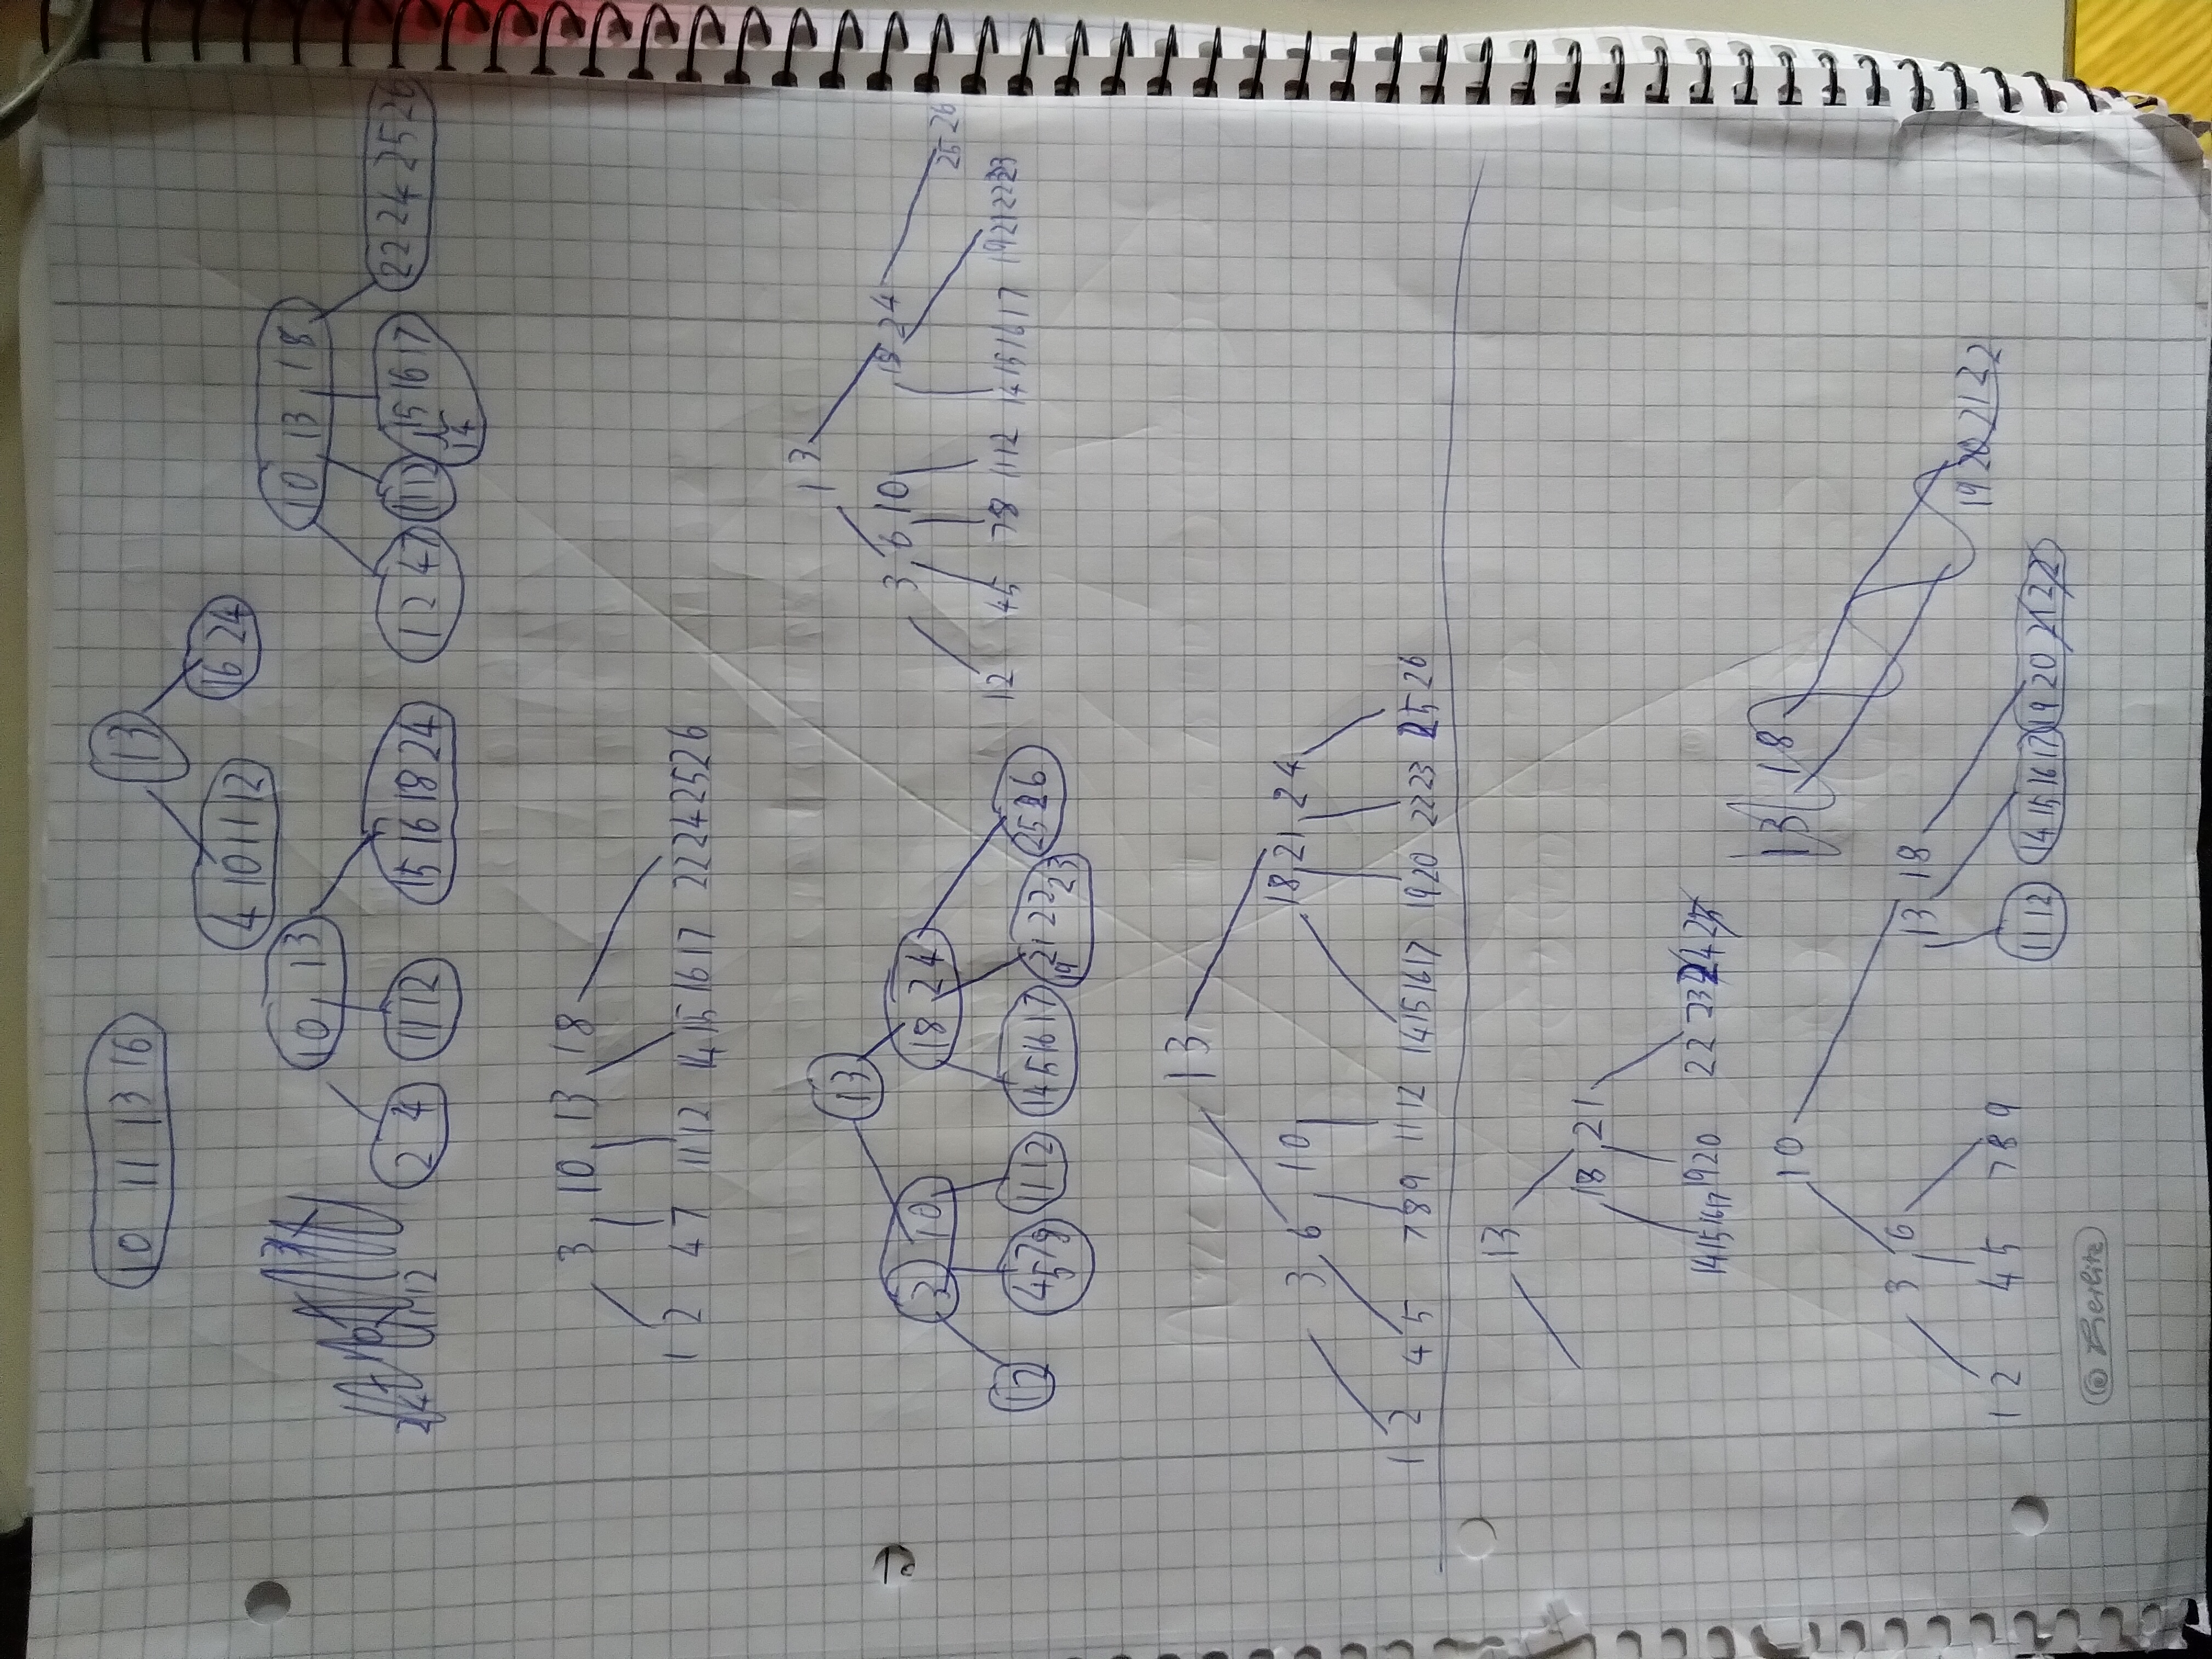
\includegraphics[height=\textwidth, angle=-90]{b_tree1}
    \centering
\end{figure}
\begin{figure}
    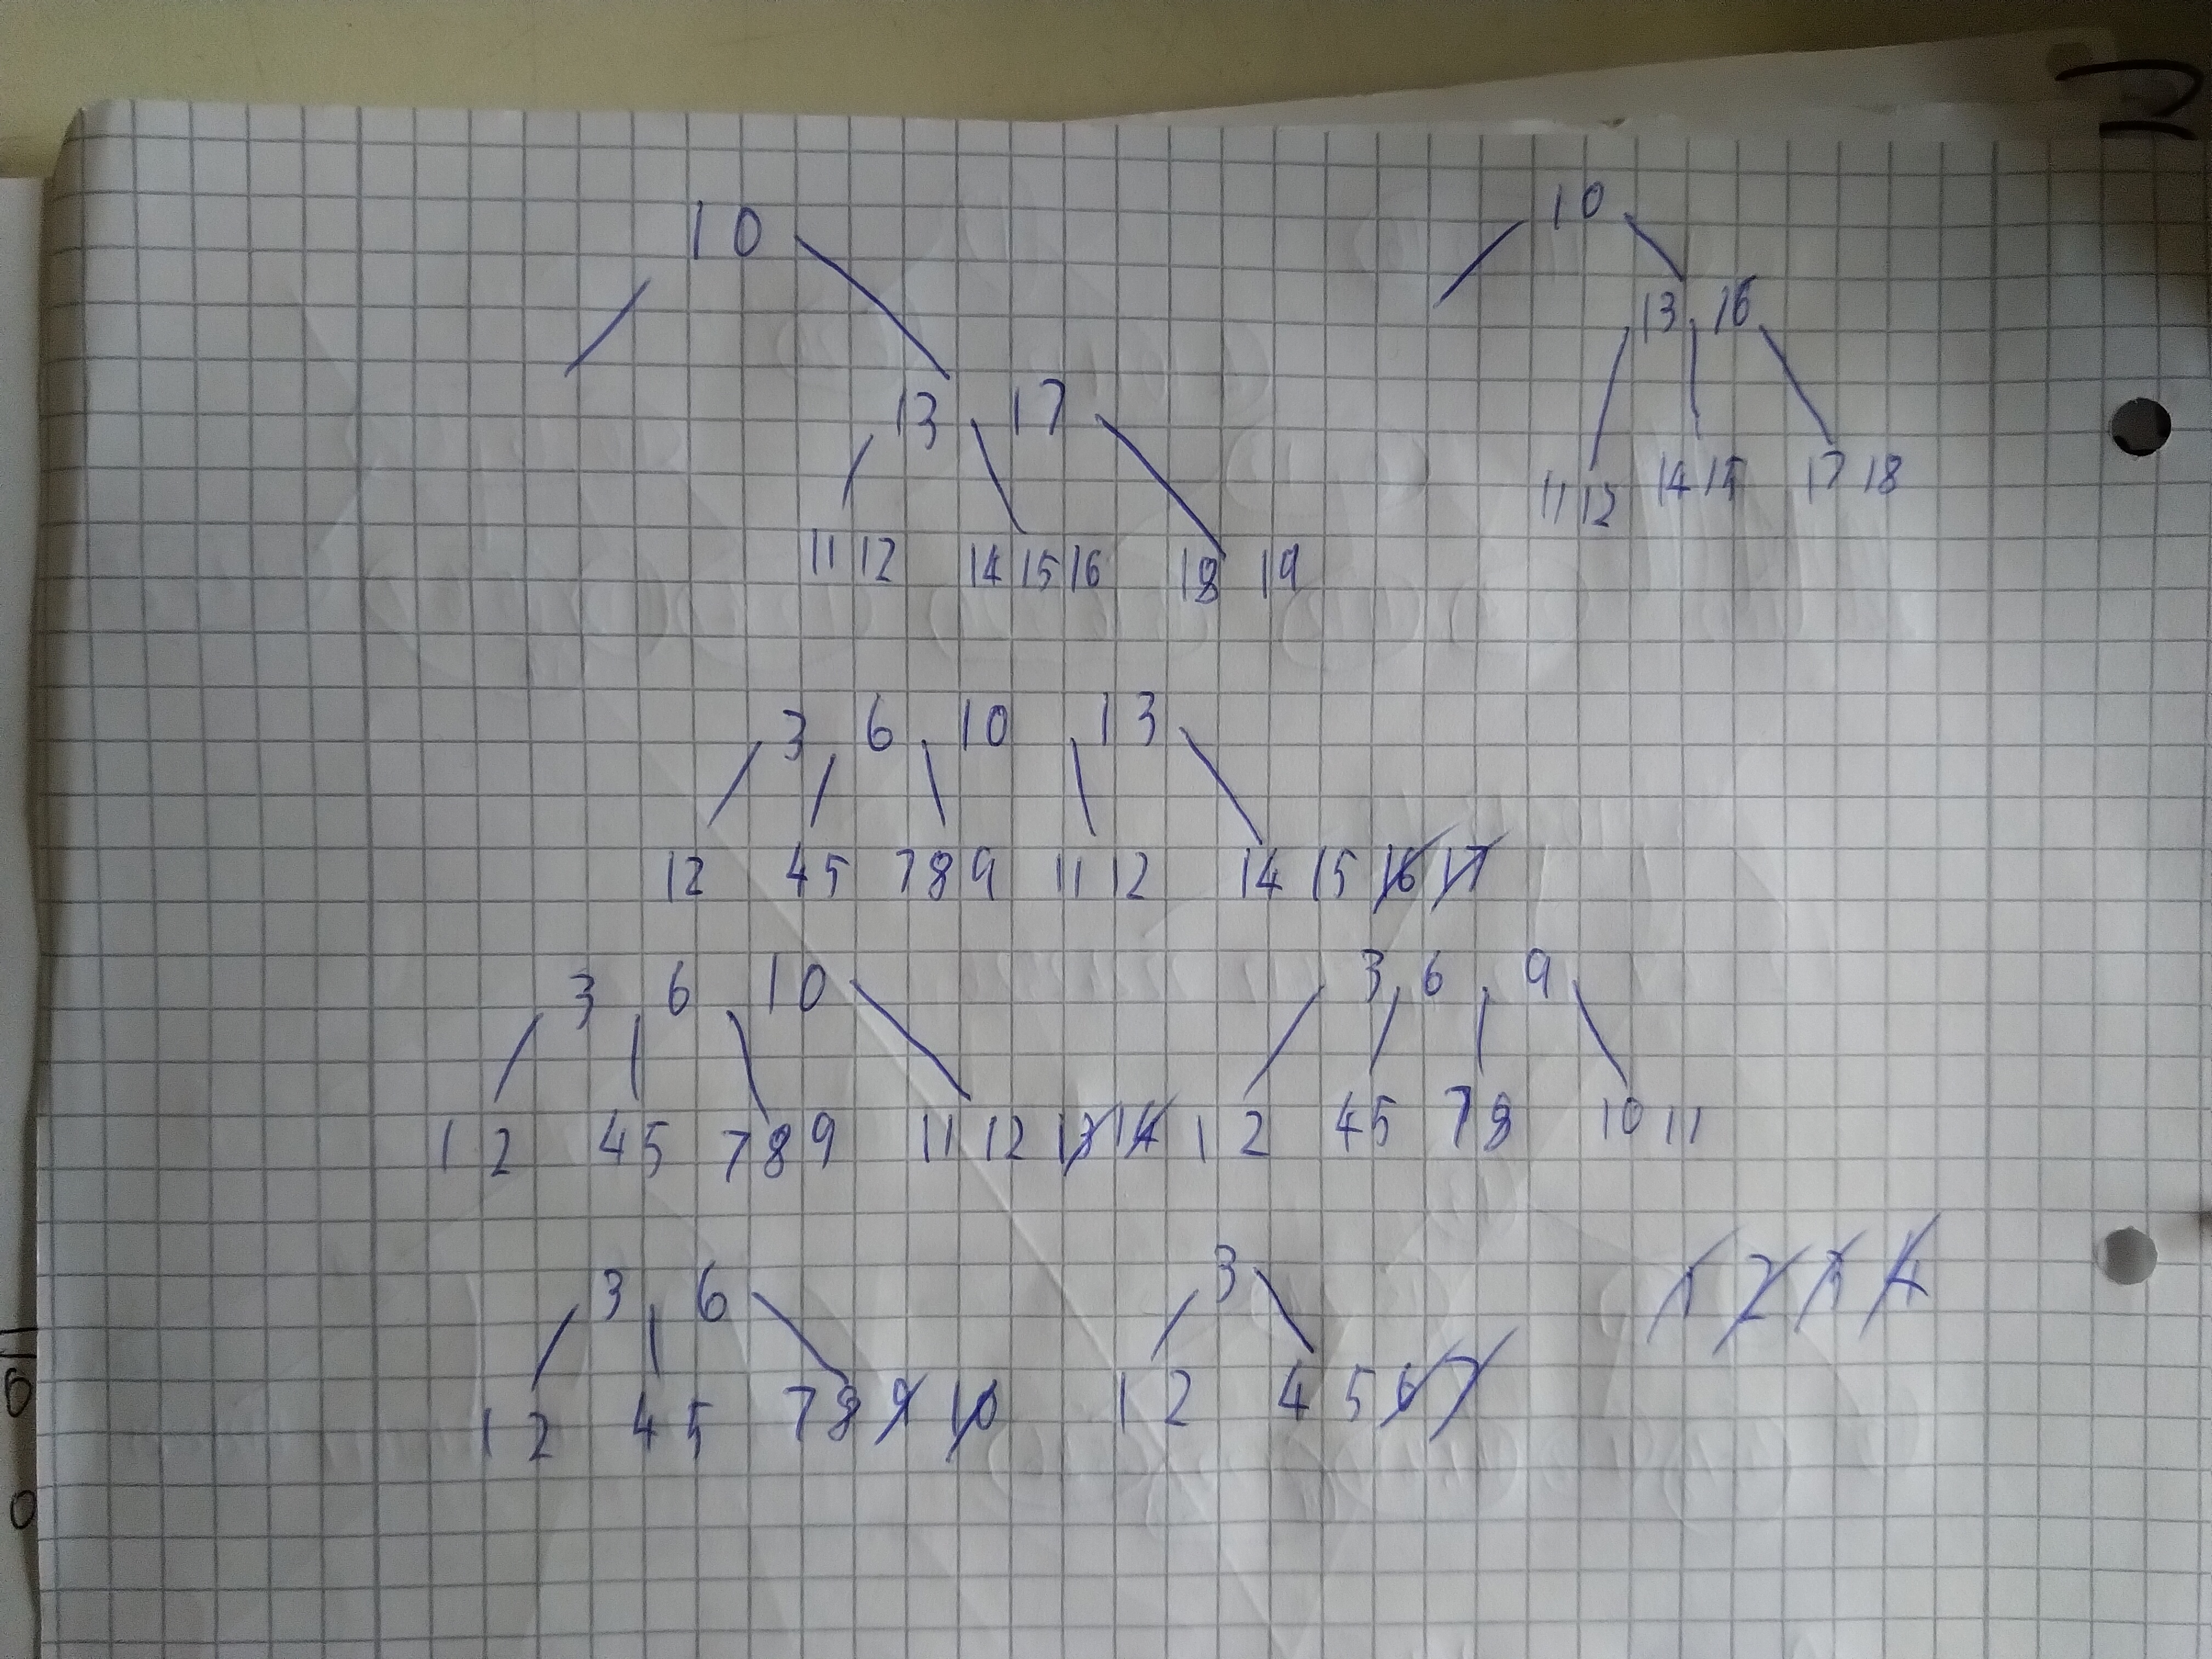
\includegraphics[width=\textwidth]{b_tree2}
    \centering
\end{figure}

\end{document}